% !TEX root = ../MasterThesis.tex

\chapter{EBES実験におけるバックグラウンド測定} \label{sec:EBES}
未確認粒子であるALPsの探索を目的としたEBES実験を行うにあたって、バックグラウンド測定を実施した。本章ではその概要と結果を報告する。

5.1節では実験に使用するビームラインKEK Linacについて述べる。5.2節では実験本番に予定している実験セットアップを説明する。5.3節では2022年7月に行ったバックグラウンド測定の概要とその結果を示す。
%\section{実験本番のセットアップ}

\section{KEK Linac}
本実験はKEKにあるLinacの第3スイッチヤードにおいて実験を予定している。
%%%%%%%%%%%%%%%%%%%%%%%%%%%%%%%%%%%%%%%%%%%%%
\begin{comment}
LinacはSuperKEKBの前段加速器であり、その概形を図\ref{SuperKEKB}に示す。
\begin{figure}[H]
	\begin{center}
		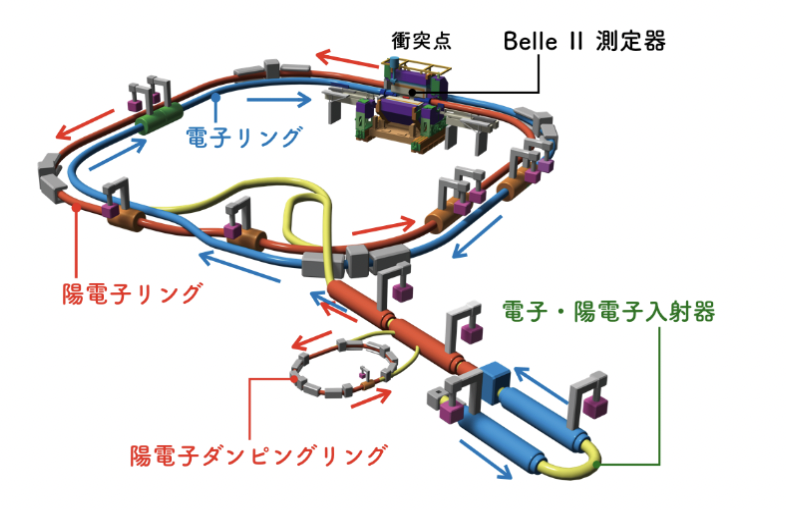
\includegraphics[width=250pt]{./Figure/EBES/SuperKEKB.png}
		\caption[SuperKEKB加速器]{SuperKEKB加速器。}
		\label{SuperKEKB}
	\end{center}
\end{figure}
\end{comment}
%%%%%%%%%%%%%%%%%%%%%%%%%%%%%%%%%%%%%%%%%%%%%
本ビームラインでは、エネルギーが最大$\SI{7}{GeV}$の電子ビームおよび$\SI{4}{GeV}$の陽電子ビームが利用可能である。%Super KEKBは設計ルミノシティ$8\times 10^{35}\SI{}{cm^{-2}s^{-1}}$の電子・陽電子加速器であり、ビームメインラインの周長はおよそ$\SI{3}{km}$である。
%ビームは電子・陽電子入射器で生成された後、それぞれのダンピングリングを通じてメインラインを周回する。

第3スイッチヤードはLinacビームライン終端に位置しており、この概形を図\ref{SY3}に示す。
\begin{figure}[H]
	\begin{center}
		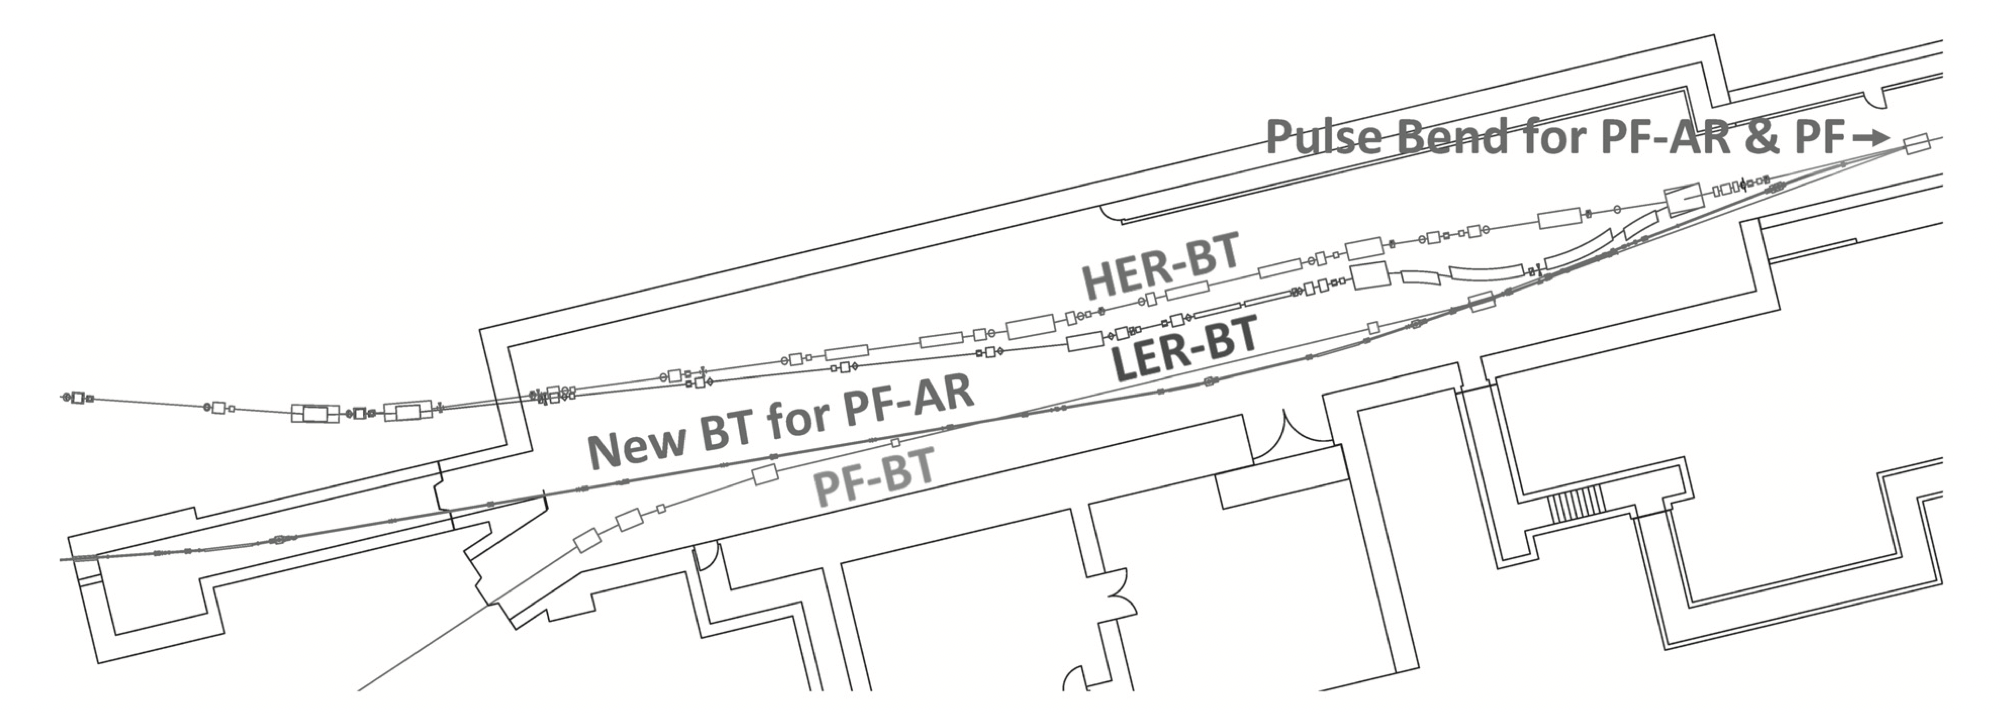
\includegraphics[width=250pt]{./Figure/EBES/SY3.png}
		\caption[第3スイッチヤード]{第3スイッチヤード。}
		\label{SY3}
	\end{center}
\end{figure}

第3スイッチヤード入口と第3スイッチヤードにはPF/PF-AR用のビーム輸送路へビームを選択的に導くパルス偏向電磁石とSuperKEKB HER/LER に入射する電子、陽電子ビームを分離する偏向電磁石とビームダンプにビームを導くための偏向電磁石が設置してある。第3スイッチヤード入口まで輸送されてきたビームはビームの輸送先に応じてパルス偏向電磁石と偏向電磁石の電流値が設定される。ビームダンプは SuperKEKB HER 用のビームラインから分岐したビームラインのため、SY3ビームダンプを使った実験はビームダンプ専用の運転に切り替えて行う。
SY3で実験を行う長所として、高いエネルギー(最大7 GeV)と高いビーム繰り返し(最大50 Hz)、可変なバンチチャージ(最大 4 nC)が挙げられる。高いエネルギーによりALPsが相対論的にブーストされ、寿命を伸ばすことができる。また、高ビーム繰り返しにより高い統計量を得ることができるため、小さい結合定数であったとしても探索に貢献できる可能性が高まる。そして、バンチチャージを変更することでバックグラウンドの割合をコントロールできる。

\section{実験セットアップ}
本実験において重要となるのがミューオンや中性子などによって生じるバックグラウンドであり、実験セットアップには十分バックグラウンドイベントを低減できるような工夫が必要となる。本実験で予定している検出器セットアップは2種類あり、それぞれセットアップ1、セットアップ2と呼ぶ。その模式図を図\ref{EBES_1}、\ref{EBES_2}に示す。
\begin{figure}[H]
	\begin{center}
		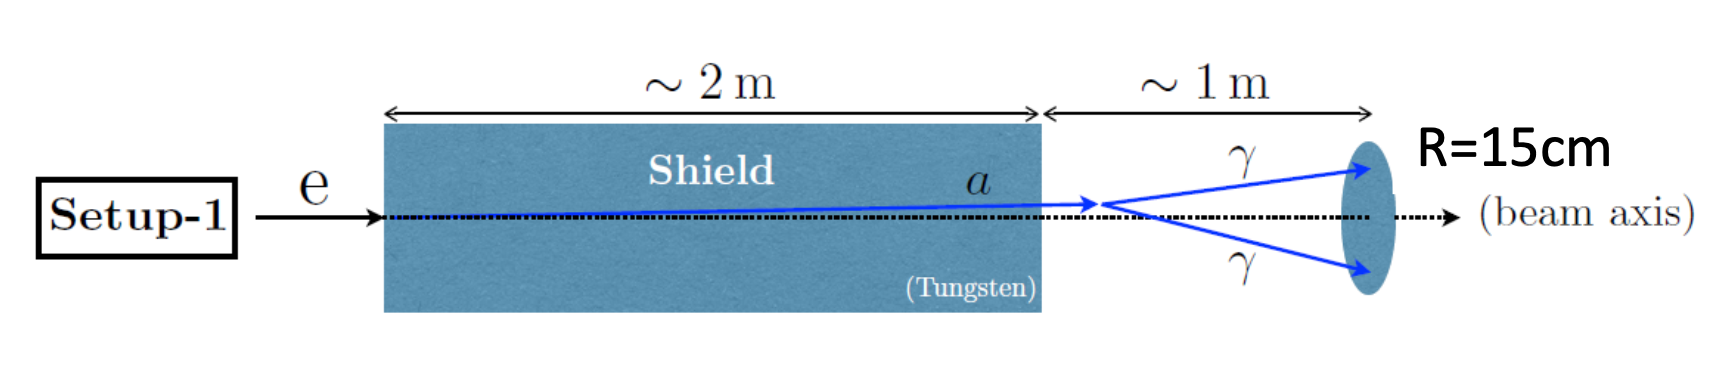
\includegraphics[width=270pt]{./Figure/EBES/EBES_1.png}
		\caption[EBES実験セットアップ1]{EBES実験セットアップ1。}
		\label{EBES_1}
	\end{center}
\end{figure}

\begin{figure}[H]
	\begin{center}
		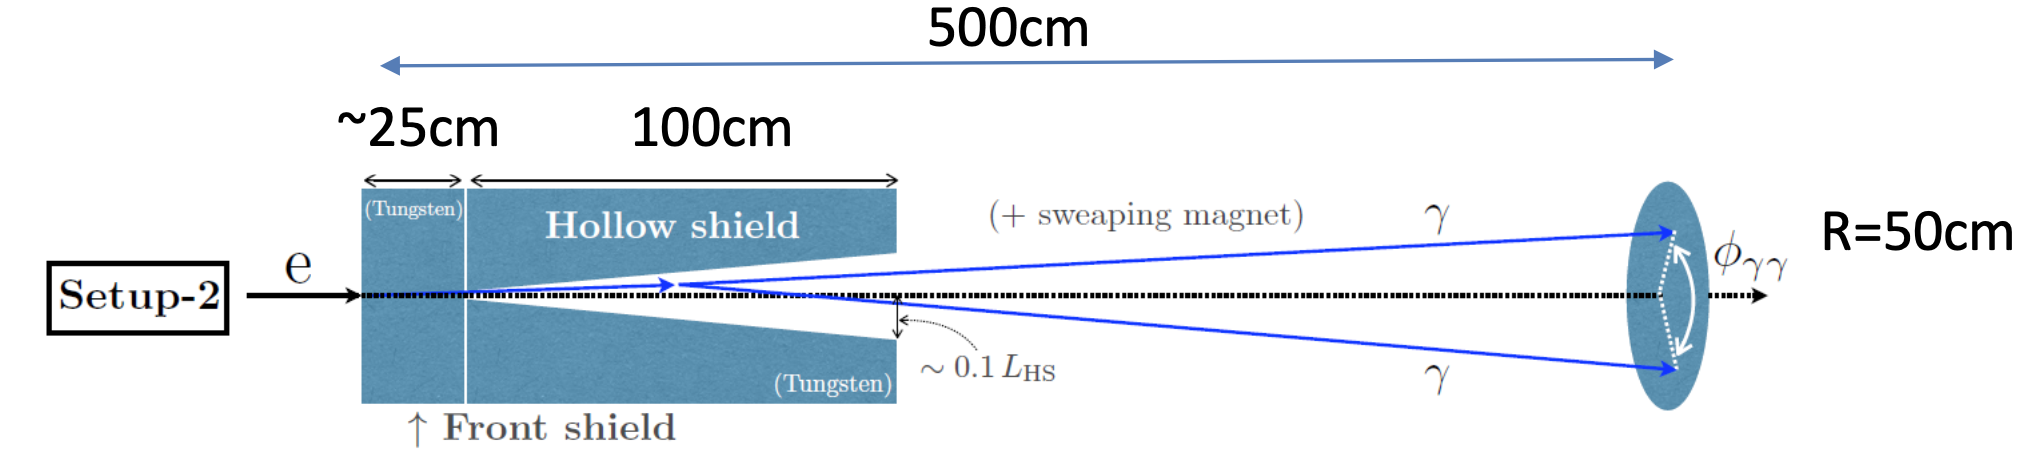
\includegraphics[width=330pt]{./Figure/EBES/EBES_2.png}
		\caption[EBES実験セットアップ2]{EBES実験セットアップ2。一部のシールドを除去し、磁場を印加している。}
		\label{EBES_2}
	\end{center}
\end{figure}


図\ref{EBES_1}にセットアップ1の模式図を示す。バックグラウンド除去のためにビームダンプ全体をタングステンシールドで遮蔽する。ビームダンプから\SI{1}{m}ほどの距離に置いた検出器で2光子事象を観測する。

図\ref{EBES_2}に示したのがセットアップ2である。シールドを一部除去し、ミューオンを偏極電磁石によって掃引する。
今回目的とするような結合定数の小さい反応をとらえる上でできるかぎりバックグラウンドイベントを低減させることが重要となる。


\section{バックグラウンド測定}
本実験を行う準備として、同じビームラインにおいてテストビームを用いた最初のバックグラウンド測定を行った。5.2.1節では、そのセットアップについて、5.2.2節ではその結果について説明する。

\subsection{バックグラウンド測定のためのセットアップ}
本実験は2022年7月11日から12日まで行われた。%ビームラインの軸上にビームダンプを設置し、図\ref{EBES_det}のように鉛ガラス検出器を設置した。
ステージを2つ用意し、それぞれビームダンプステージおよび検出器ステージとして利用した。ビームダンプとして鉛および鉄を設置し、その上部に鉛ガラス検出器を配置した。検出器ステージの上にはSiW ECALレイヤーを1台設置し、その後ろに鉛ガラス検出器を5台設置した。SiW ECALは本実験においてバックグラウンド削減のために使用されるが、今回の測定ではタングステンを設置していないため荷電粒子の識別を意図して設置した。

\begin{figure}[H]
	\begin{center}
		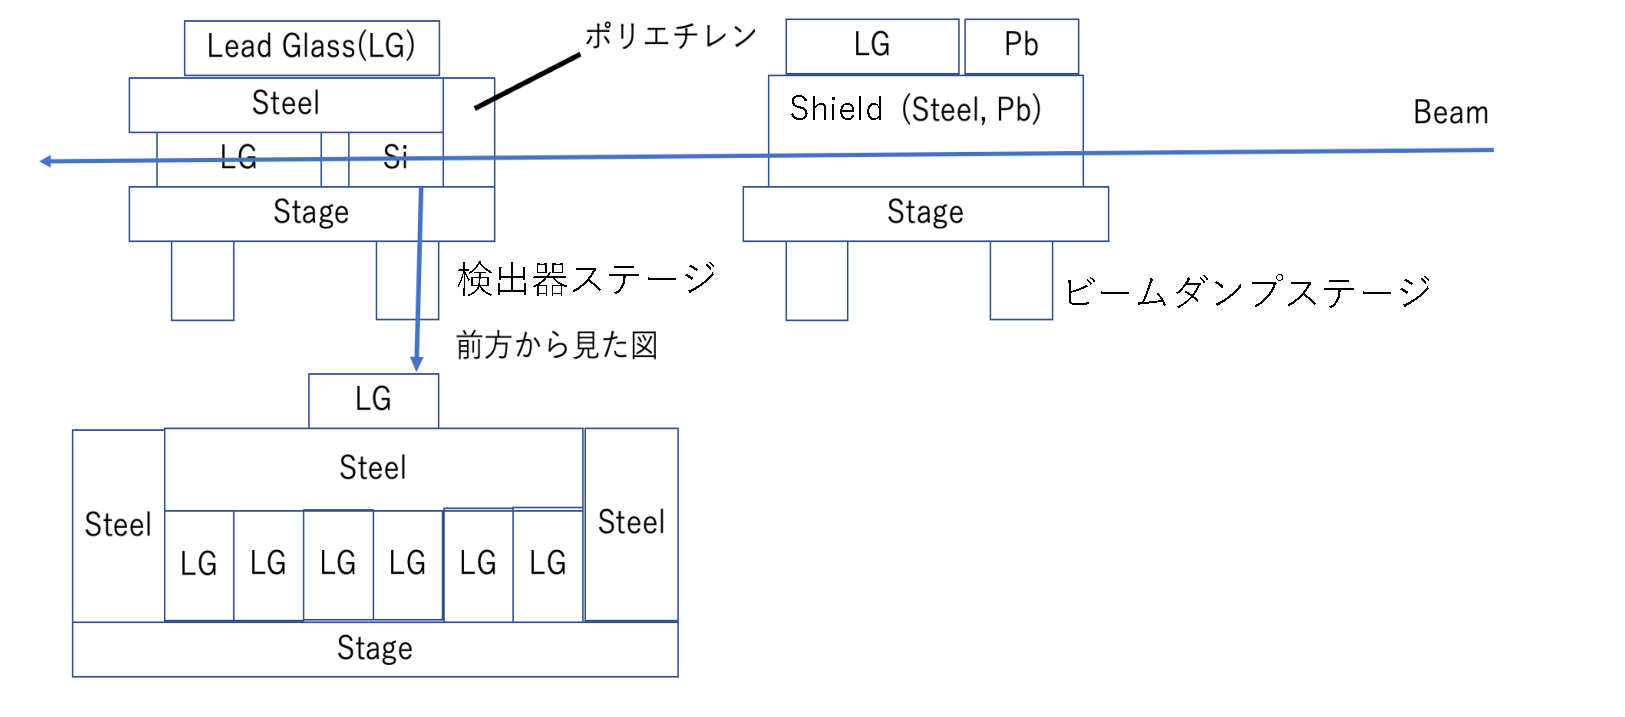
\includegraphics[width=330pt]{./Figure/EBES/EBES_det.pdf}
		\caption[バックグラウンド測定のためのセットアップ]{バックグラウンド測定のためのセットアップ。LGが鉛ガラス検出器、SiがSiW ECALレイヤー、Pb、Steelはそれぞれ遮蔽のための鉛および鉄ブロック、Stageはステージである。}
		\label{EBES_det}
	\end{center}
\end{figure}


鉛ガラス検出器およびSiW ECALにより生じた信号は、別室に接続されたPCへとデータが送信される。鉛ガラス検出器にはNIMモジュールを用いた論理回路を作成し、CAMAC PCによるデータ記録を行った。SiW ECALについてはSLボードに接続されたUSBケーブルによって直接PCへとデータが送信される。

電子および陽電子ビームの輸送は図\ref{EBES_beam1}および\ref{EBES_beam2}のように行われる。図(a)と図(b)は接続しており、両方の図に含まれる四極DC電磁石QF61A1は同じものである。偏向電磁石で軌道を曲げられたビームは四重極電磁石によって収束された後、再度偏向電磁石に曲げられビームダンプへと衝突する。

\begin{figure}[H]
		%\begin{center}
 		 	\includegraphics[width=400pt]{./Figure/EBES/EBES_beam1.png}%.5\linewidth]{./Figure/DLAnalysis/Input2.png}
 		%\end{center}
	\caption[加速器セットアップの模式図]{加速器セットアップの模式図。}
	\label{EBES_beam1}
\end{figure}

\begin{figure}[H]
		%\begin{center}
 		 	\includegraphics[width=400pt]{./Figure/EBES/EBES_beam2.png}%.5\linewidth]{./Figure/DLAnalysis/Input2.png}
   		%\end{center}
	\caption[加速器セットアップの模式図2]{加速器セットアップの模式図2。}
	\label{EBES_beam2}
\end{figure}



ビーム生成方法として、RF(radio frequency, 高周波)および熱電子銃を使用し、ビームの種類やビーム繰り返し、ビームエネルギーを変化させて検出器応答を確認した。表\ref{EBES_run}は長時間データを記録できた主な測定時間を示している。鉛ガラス検出器に印加する電圧やCAMACチャンネルとの対応は適宜変更されている。

%$測定時間[\SI{}{min} : 表に追加しようと思ったがランリストに一部記録していなかったのでやめた

\begin{table}[h]
	\begin{center}
		\begin{tabular}{|cccc|}
		\hline
		測定開始時刻&ビーム種類&ビームエネルギー[\SI{}{GeV}]&ビーム周波数[\SI{}{Hz}]\\\hline\hline
		2022/7/11  6:12&陽電子&4.0&25\\\hline
		2022/7/11  6:47&陽電子&4.0&25\\\hline
		2022/7/11  8:26&電子&7.0&1.0\\\hline
		2022/7/11 10:41&電子&7.0&25-5 \\\hline
		2022/7/11 17:44&陽電子&4.0&25\\\hline
		%2022/7/11 20:30&陽電子&4.0&25\\\hline
		\end{tabular}
	\end{center}
	\caption[長時間測定できた鉛ガラス検出器のrunのリスト]{長時間測定できた鉛ガラス検出器のrunのリスト}
\label{EBES_run}
\end{table}

それぞれのビームタイムをビームタイム1-5とした。

\subsection{結果}

ビーム位置モニターにより測定されたビームの位置および電荷と鉛ガラス検出器の応答を比較することで、ビーム位置とバックグラウンドイベントの依存性を確認した。ビームの位置は図\ref{EBES_beam1}の鉄心DCマグネットBX61H1および偏向電磁石BM61A1の付近に置かれたビーム位置モニターにより測定されている。以下それぞれSP61H1およびSP61A1とする。

表\ref{EBES_run}の時間ごとに測定された、ビーム位置と鉛ガラス検出器の応答の依存性が図\ref{EBAS_Beam_dep_1} - \ref{EBAS_Beam_dep_5}に示されている。

\begin{figure}[H]
	\begin{center}
		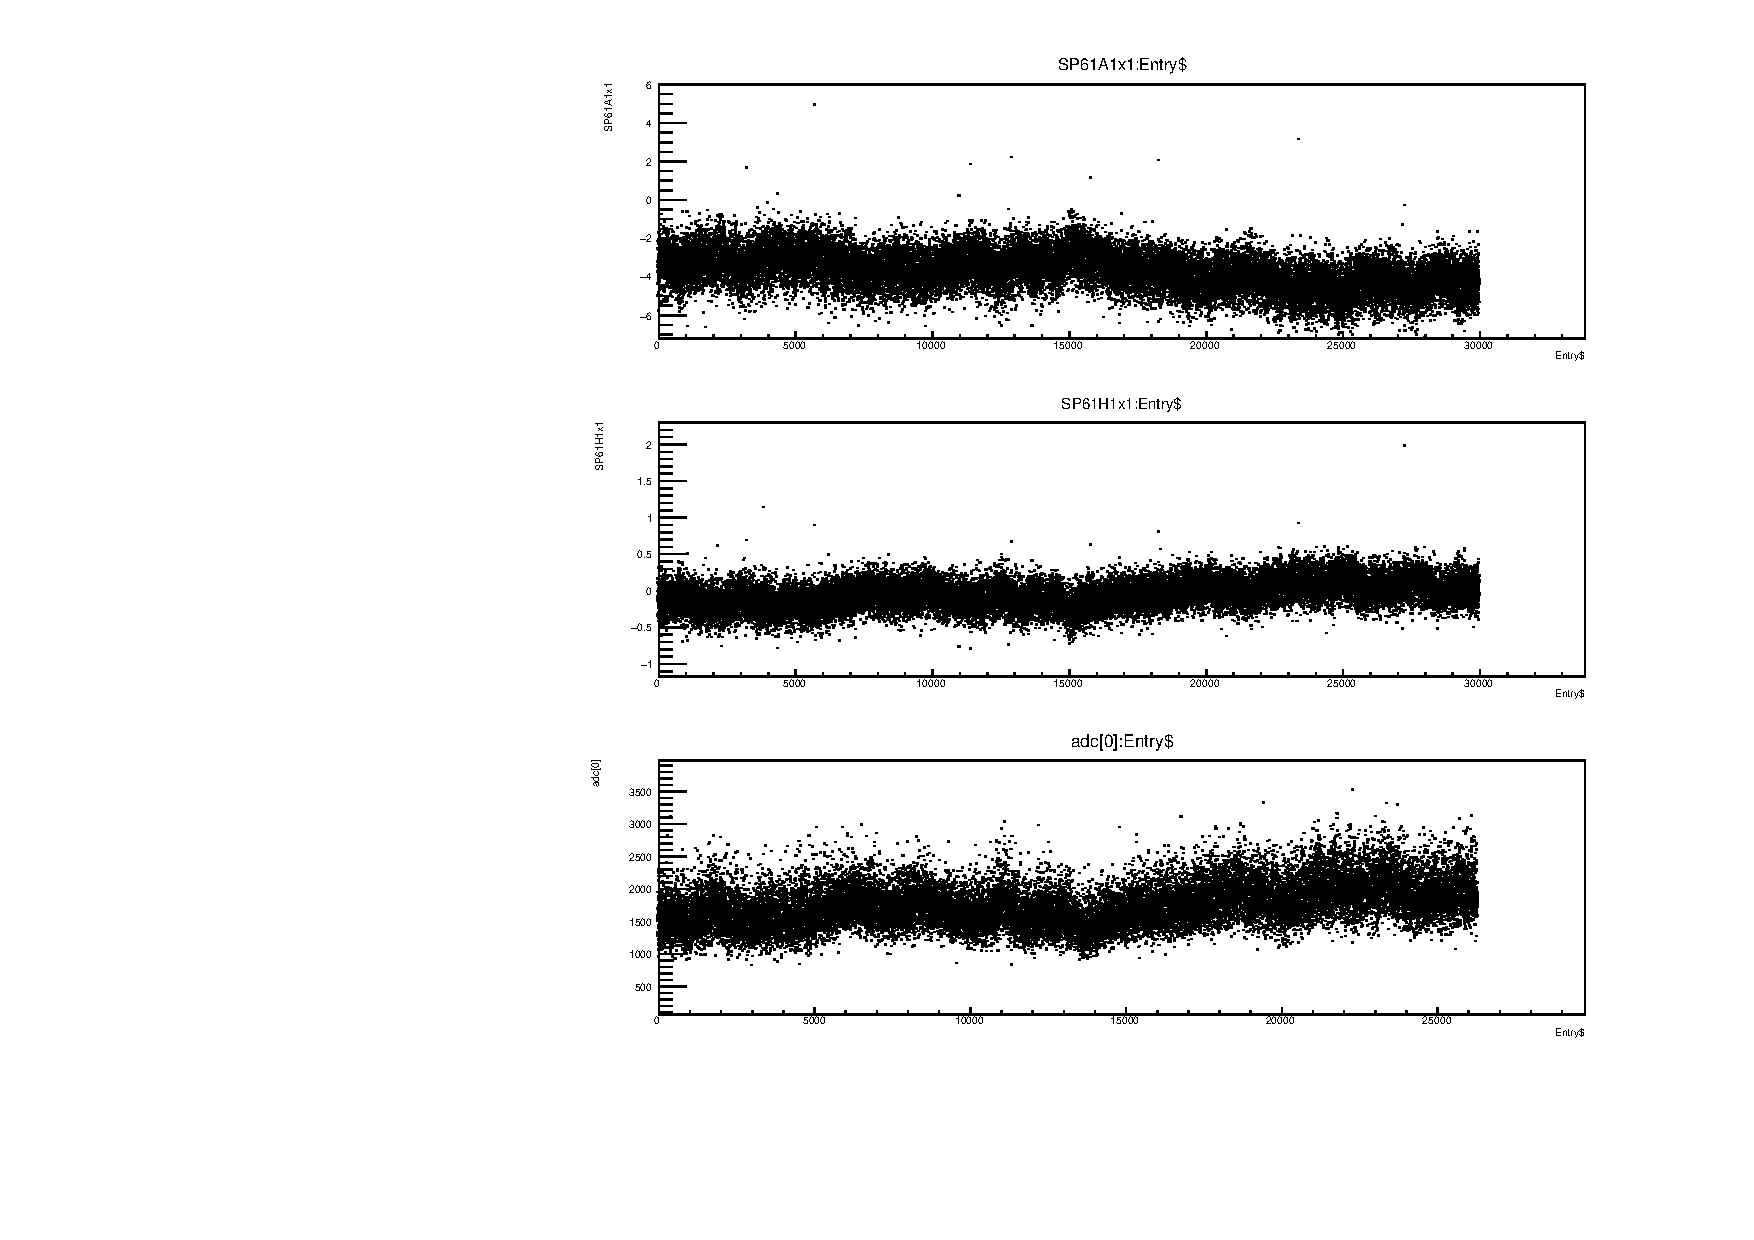
\includegraphics[width=330pt]{./Figure/EBES/BPB_dep1.pdf}
		\caption[ビームタイム1におけるビーム位置と鉛ガラス検出器の応答の依存性]{ビームタイム1におけるビーム位置と鉛ガラス検出器の応答の依存性。一番上の図がSP61A1を通過したビームの$x$座標、真ん中の図がSP61H1を通過したビームの$x$座標、一番下の図が鉛ガラス検出器の応答である。}
		\label{EBAS_Beam_dep_1}
	\end{center}
\end{figure}

\begin{figure}[H]
	\begin{center}
		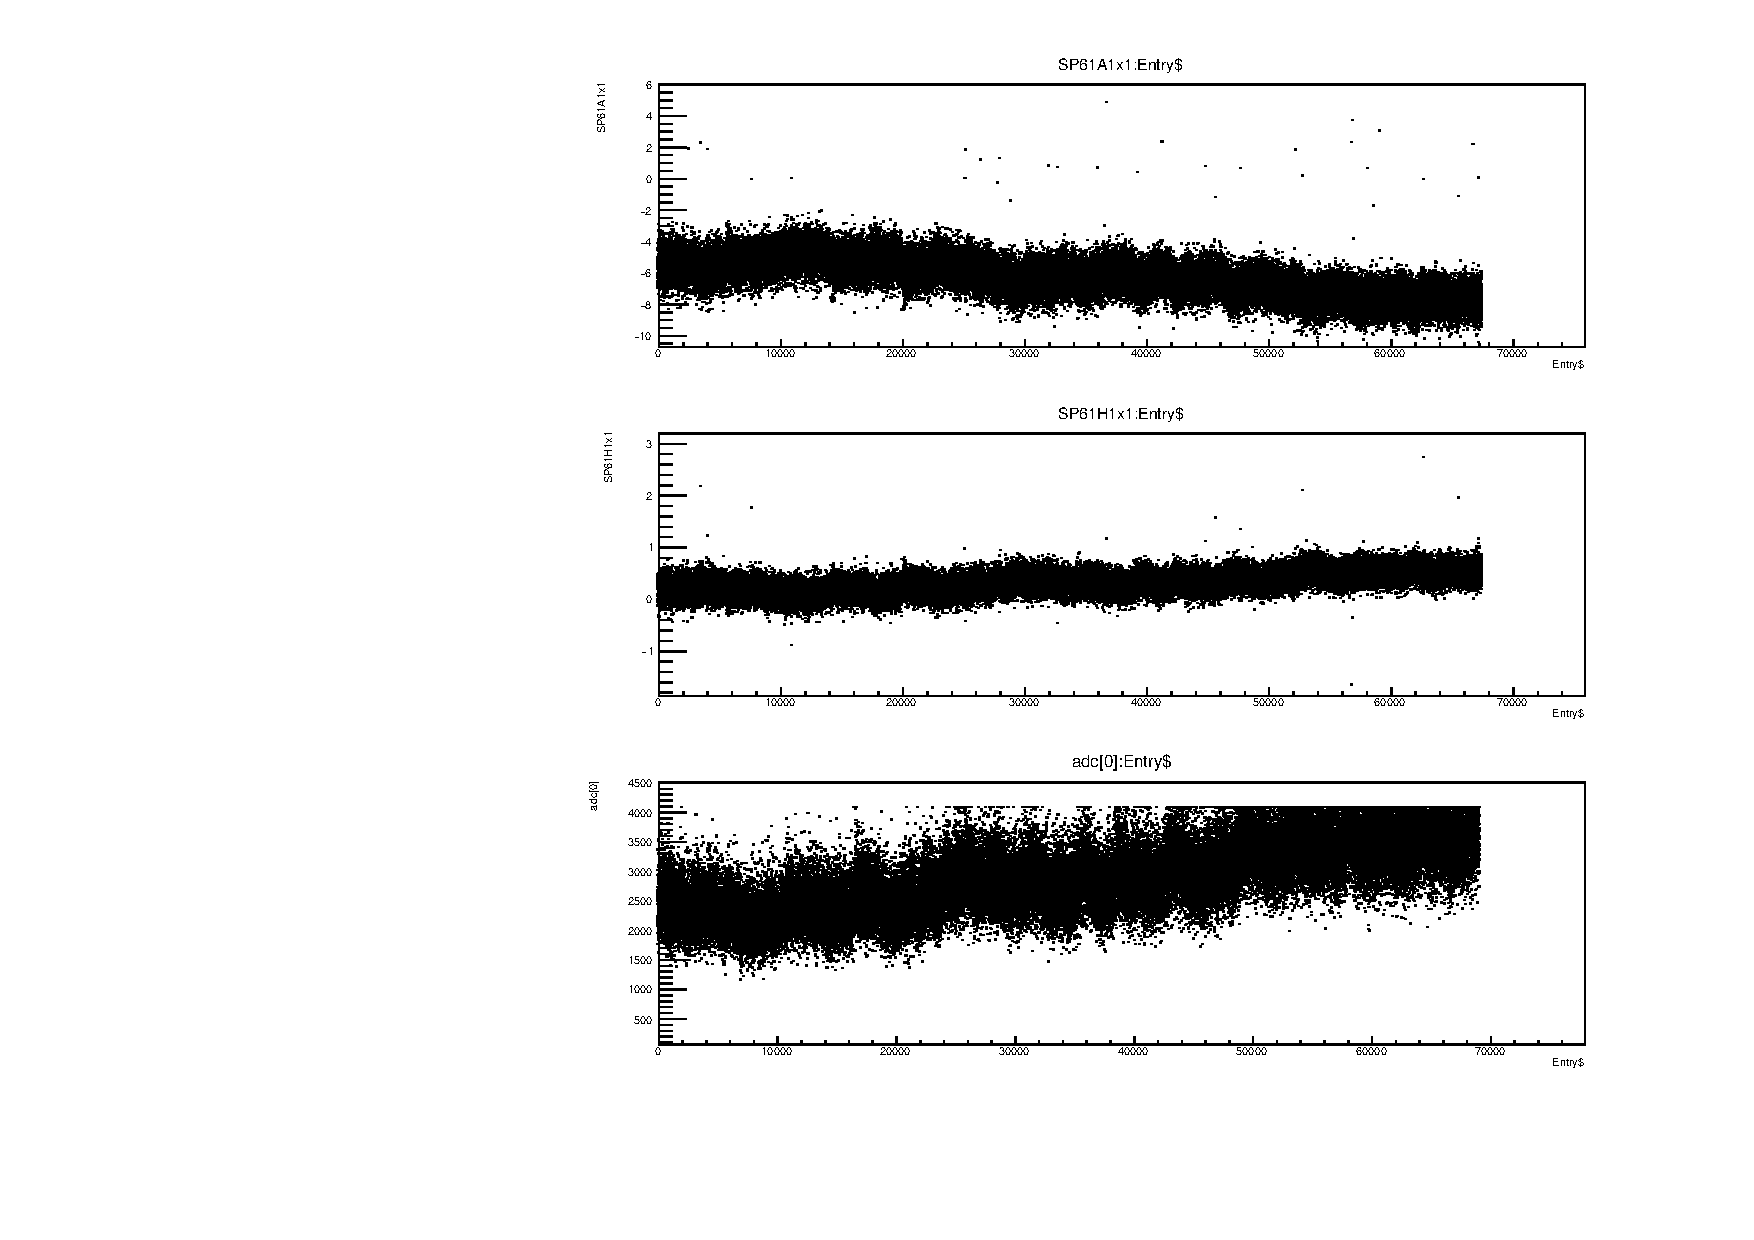
\includegraphics[width=330pt]{./Figure/EBES/BPB_dep2.pdf}
		\caption[ビームタイム2におけるビーム位置と鉛ガラス検出器の応答の依存性]{ビームタイム2におけるビーム位置と鉛ガラス検出器の応答の依存性。一番上の図がSP61A1を通過したビームの$x$座標、真ん中の図がSP61H1を通過したビームの$x$座標、一番下の図が鉛ガラス検出器の応答である。}
		\label{EBAS_Beam_dep_2}
	\end{center}
\end{figure}

\begin{figure}[H]
	\begin{center}
		\includegraphics[width=330pt]{./Figure/EBES/BPB_dep3.pdf}
		\caption[ビームタイム3におけるビーム位置と鉛ガラス検出器の応答の依存性]{ビームタイム3におけるビーム位置と鉛ガラス検出器の応答の依存性。一番上の図がSP61A1を通過したビームの$x$座標、真ん中の図がSP61H1を通過したビームの$x$座標、一番下の図が鉛ガラス検出器の応答である。}
		\label{EBAS_Beam_dep_3}
	\end{center}
\end{figure}

\begin{figure}[H]
	\begin{center}
		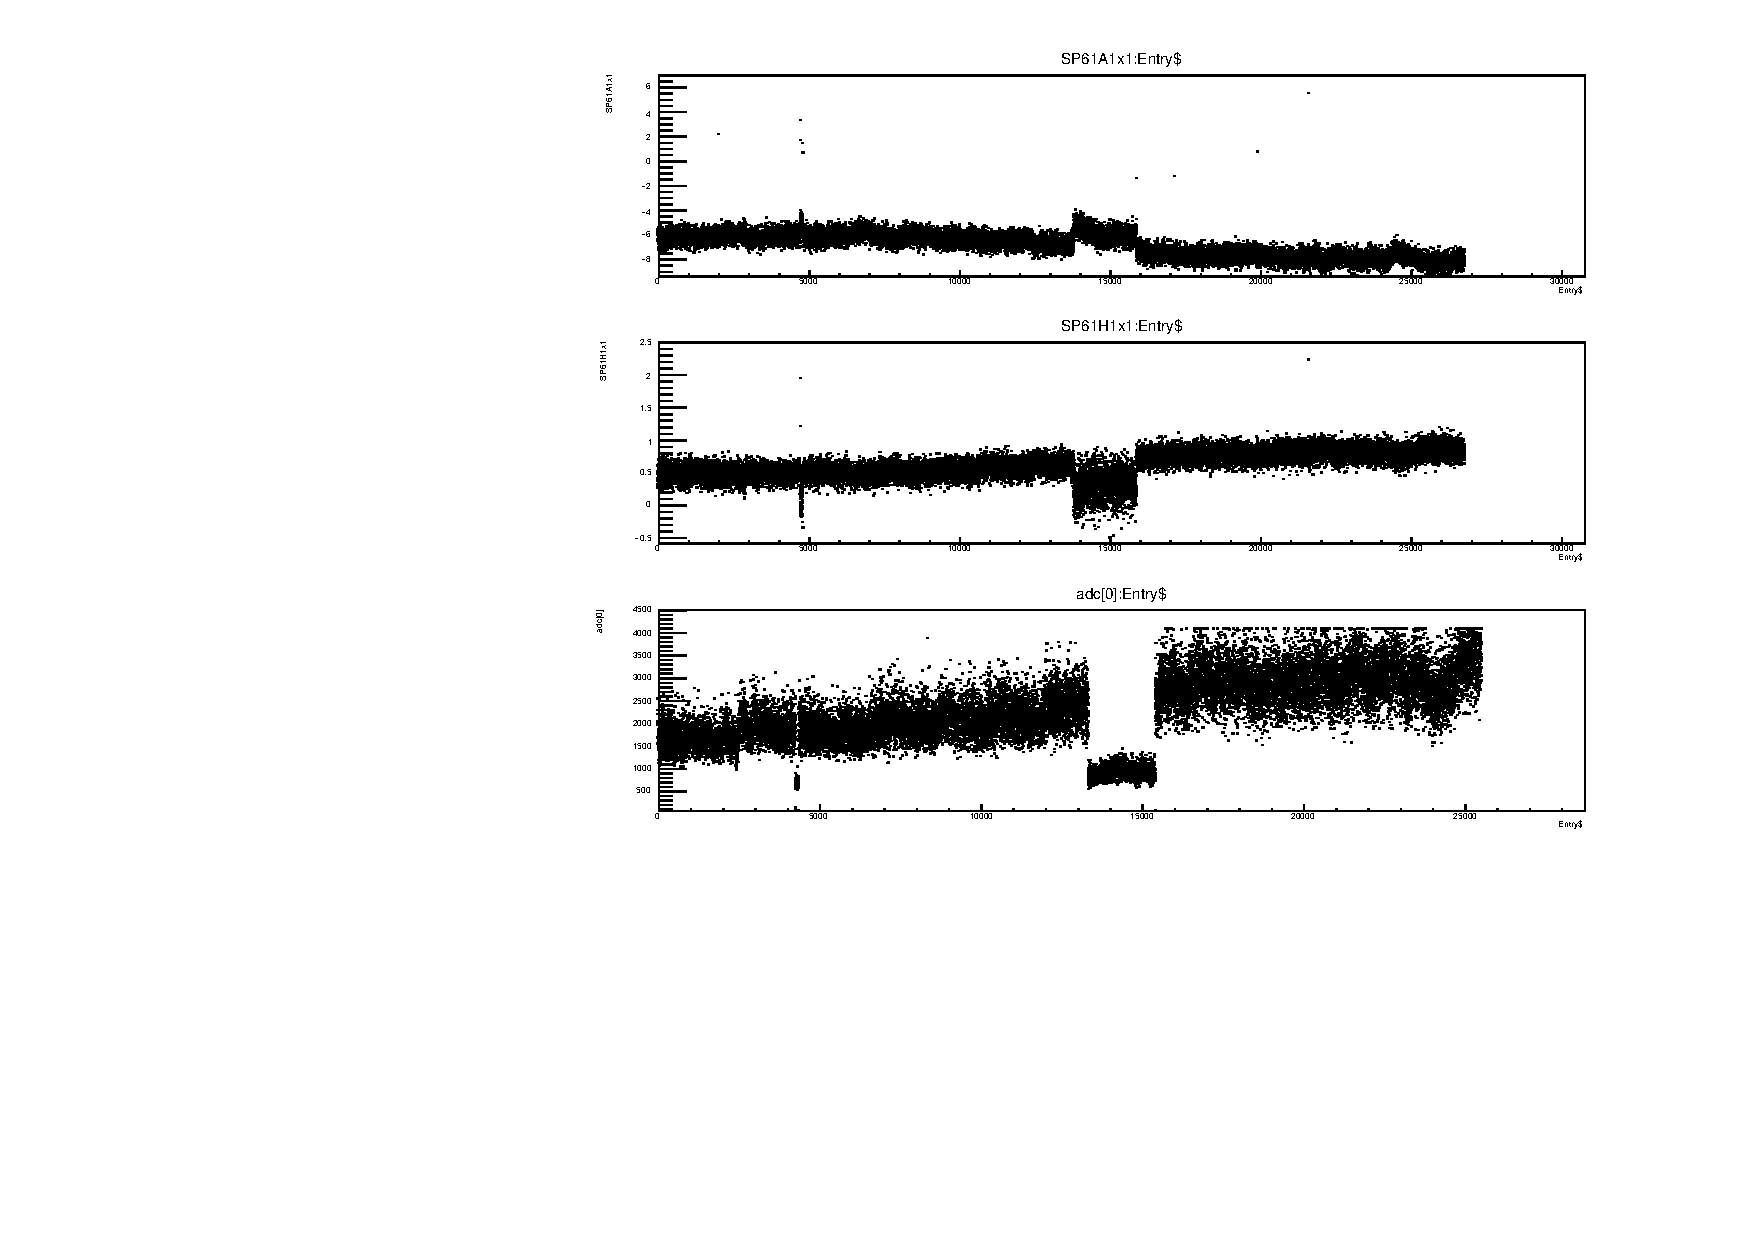
\includegraphics[width=330pt]{./Figure/EBES/BPB_dep4.pdf}
		\caption[ビームタイム4におけるビーム位置と鉛ガラス検出器の応答の依存性]{ビームタイム4におけるビーム位置と鉛ガラス検出器の応答の依存性。一番上の図がSP61A1を通過したビームの$x$座標、真ん中の図がSP61H1を通過したビームの$x$座標、一番下の図が鉛ガラス検出器の応答である。}
		\label{EBAS_Beam_dep_4}
	\end{center}
\end{figure}

\begin{figure}[H]
	\begin{center}
		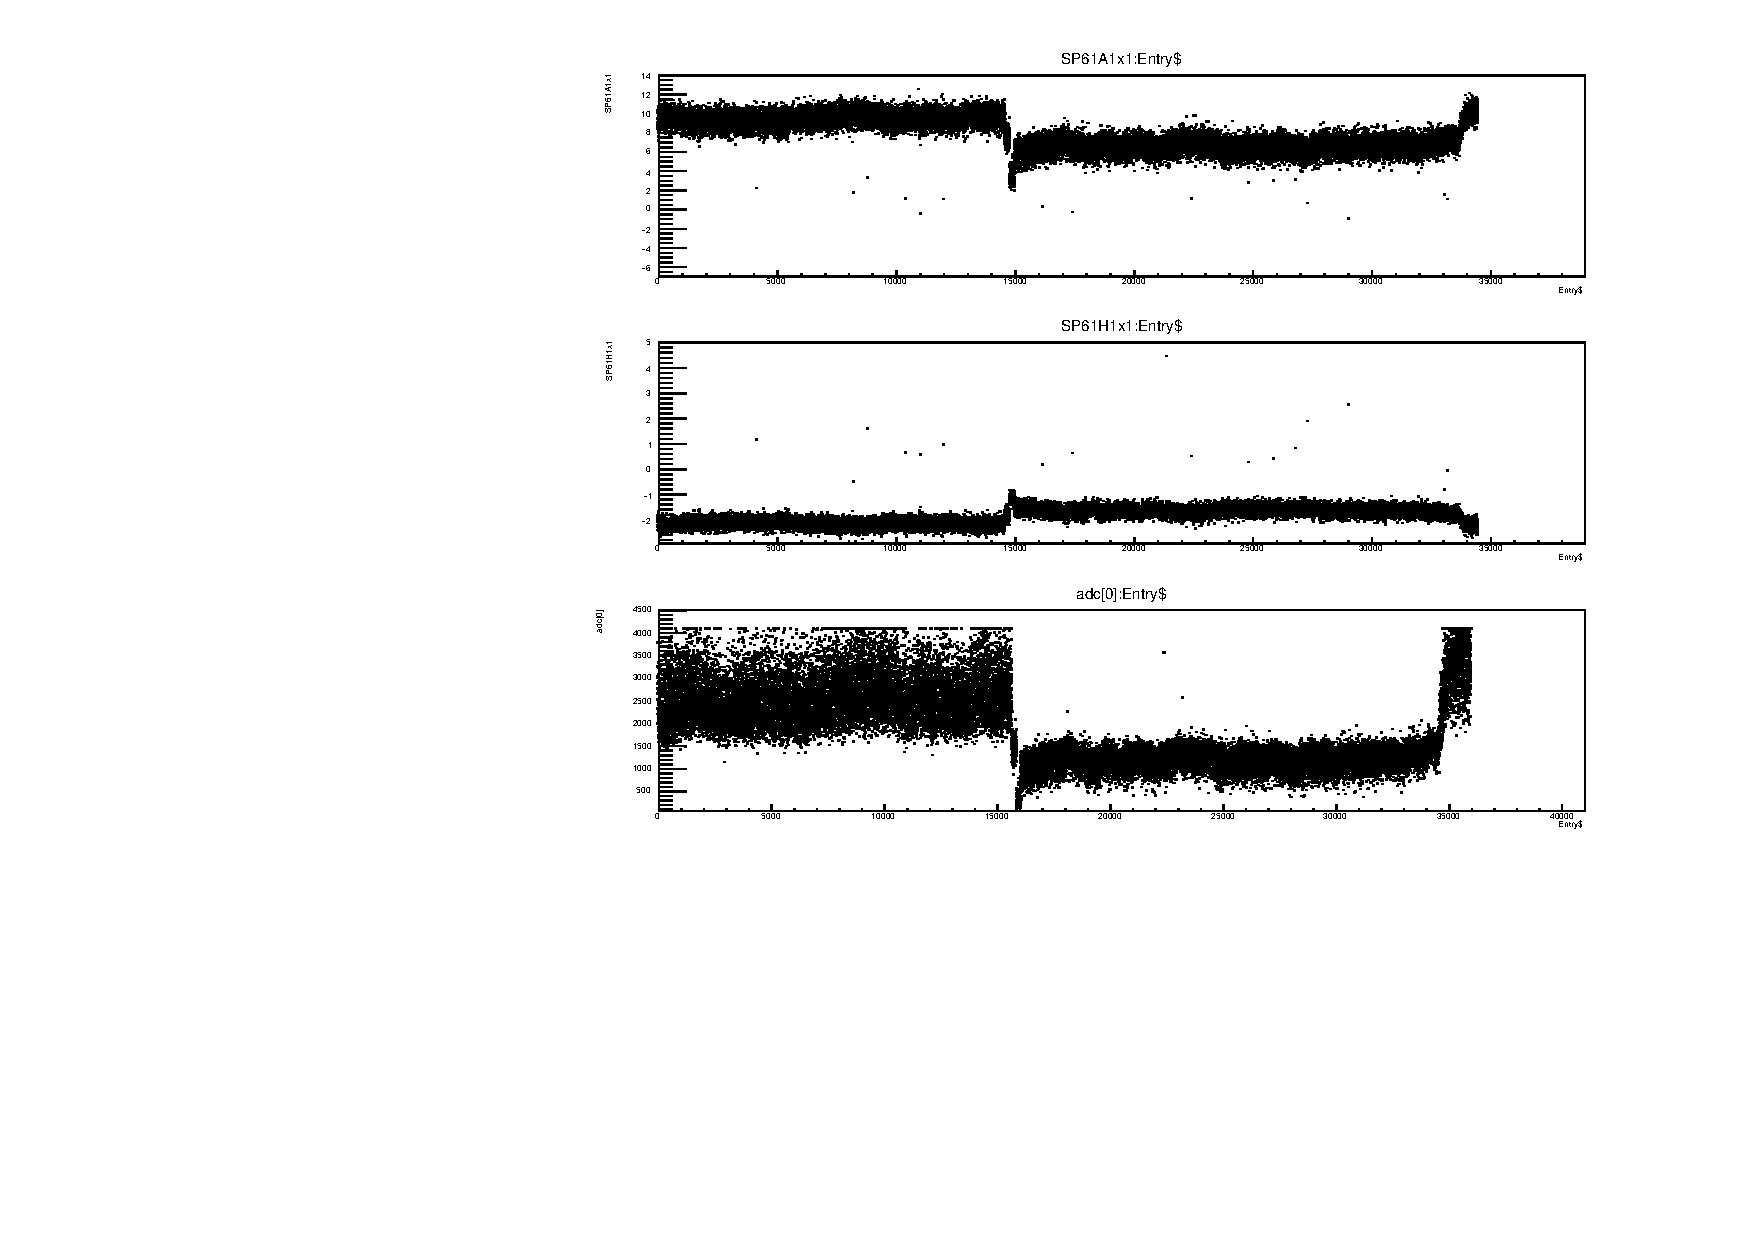
\includegraphics[width=330pt]{./Figure/EBES/BPB_dep5.pdf}
		\caption[ビームタイム5におけるビーム位置と鉛ガラス検出器の応答の依存性]{ビームタイム5におけるビーム位置と鉛ガラス検出器の応答の依存性。一番上の図がSP61A1を通過したビームの$x$座標、真ん中の図がSP61H1を通過したビームの$x$座標、一番下の図が鉛ガラス検出器の応答である。}
		\label{EBAS_Beam_dep_5}
	\end{center}
\end{figure}

%%%%%%%%%%%%%%%%%%%%%%%%%%%%%%%%%%%%%%%%%%%%%%%%%%%%%%%%%%%%%%%%%
\begin{comment}
\begin{figure}[H]
	\begin{center}
		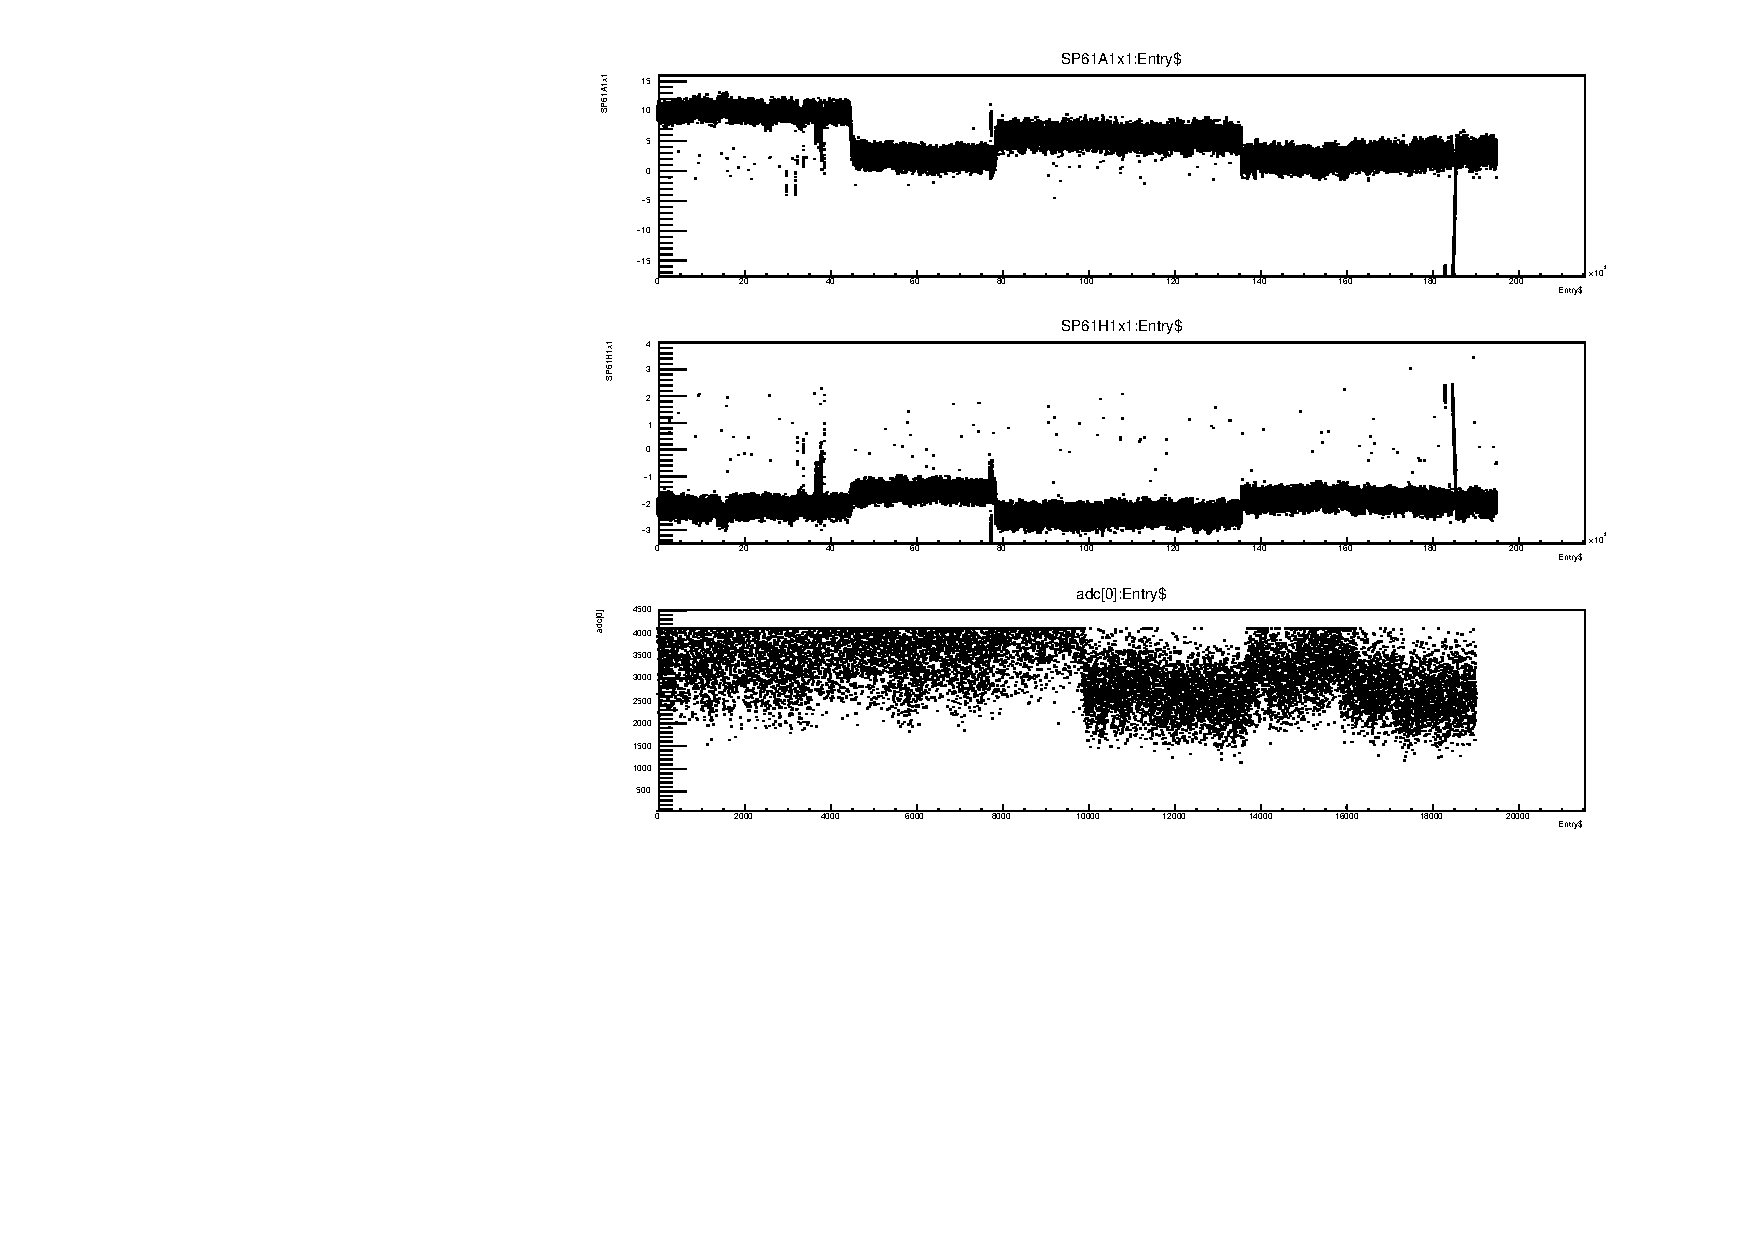
\includegraphics[width=330pt]{./Figure/EBES/BPB_dep6.pdf}
		\caption[ビームタイム6におけるビーム位置と鉛ガラス検出器の応答の依存性]{ビームタイム6におけるビーム位置と鉛ガラス検出器の応答の依存性。一番上の図が61A1にあたったビームの$x$座標、真ん中の図が61H1に通過したビームの$x$座標、一番下の図が鉛ガラス検出器の応答である。}
		\label{EBAS_Beam_dep_6}
	\end{center}
\end{figure}
\end{comment}
%%%%%%%%%%%%%%%%%%%%%%%%%%%%%%%%%%%%%%%%%%%%%%%%%%%%%%%%%%%%%%%%%%

ビームの$x$座標の揺らぎと鉛ガラス検出器の応答を比較すると、近いイベントで共通した変動が見られていることがわかる。SP61A1が$x$座標が増加すると、それに伴ってSP61H1の$x$座標が減少し、鉛ガラス検出器のADCも減少している。一方、SP61A1の$x$座標が減少すると、逆にSP61H1の$x$座標が増加し、鉛ガラス検出器のADCは増加する。このことから、SP61A1において$x$座標を減少させる方向へとビームを移動させた場合、何らかのバックグラウンドイベントが発生している可能性がある。例としてビームハローがビームパイプに衝突することによりビームロスが生じ、物質中で電子が制動放射を起こすことで生成された$\gamma$線が図\ref{background_source}のようにSP61A1とSP61H1の間で発生している可能性が示唆される。制動放射により発生した$\gamma$線はビーム軸と同じ向きに照射されやすく、加速器と測定器の位置関係から$\gamma$線が今回使用した測定器を通過しバックグラウンドとして測定された可能性がある。

\begin{figure}[H]
	%\begin{center}
	\begin{subfigure}{.9\textwidth}
 		 	\includegraphics[width=300pt]{./Figure/EBES/Background_cause1.png}%.5\linewidth]{./Figure/DLAnalysis/Input2.png}
  			\caption{}
  			\label{fig:sfig1}
	\end{subfigure}
	\begin{subfigure}{.9\textwidth}
			\includegraphics[width=300pt]{./Figure/EBES/Background_cause2.png}%.5\linewidth]{./Figure/DLAnalysis/Input2.png}
			\caption{}
			\label{fig:sfig2}
	\end{subfigure}
	%\end{center}
	\caption[バックグラウンド発生原因を表した模式図]{バックグラウンド発生原因を表した模式図。}
	\label{background_source}
\end{figure}


%定量的なバックグラウンドの発生レートを調べるためには鉛ガラス検出器をHV scan解析する必要がある。これは、HVの値を変えた時の鉛ガラス検出器応答を調べるものである。その上で鉛ガラス検出器に印加しているHVの値を参照して、バックグラウンド測定で得られたADCをHV scanで得られた信号と比較することで発生レートが概算できる。
今回用いた鉛ガラス検出器のうちの1つはHVを$\SI{850}{V}$を印加した。その検出器によって得られたADCを図\ref{background}に示す。
6章の結果を用いて検出器内に入射した粒子1つあたりのエネルギーを$\SI{1}{GeV}$と仮定すると、ADCとして1000-2500程度が検出器に入射しているため、1イベント当たりのバックグラウンド発生レートは480-1200 counts/eventとなる。これは観測のためには厳しいバックグラウンドであり、ALPを観測するために少なくとも1 count/event、ADCに換算するとおよそ2ほどまで低減させる必要がある。

\begin{figure}[H]
	\begin{center}
		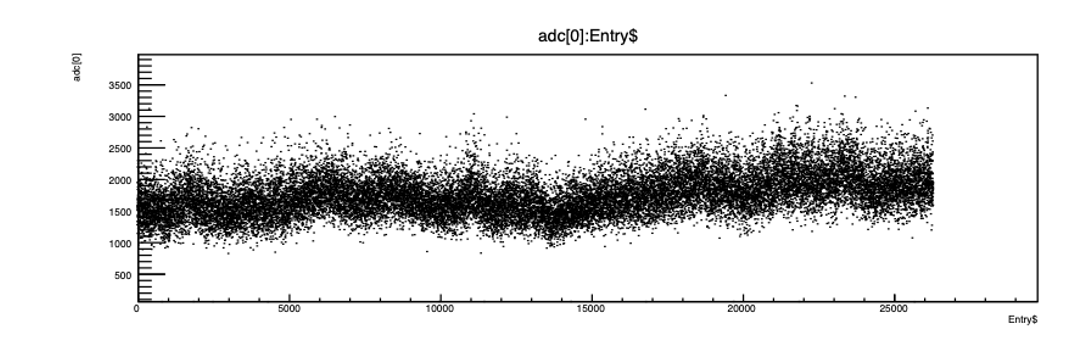
\includegraphics[width=330pt]{./Figure/EBES/background_ADC.png}
		\caption[バックグラウンド測定において得られたADCのエントリーごとの推移]{バックグラウンド測定において得られたADCのエントリーごとの推移。およそ1000 - 2500程度に分布している。}
		\label{background}
	\end{center}
\end{figure}

そのために、まずバックグラウンド発生源の遮蔽を行う。検出器から見てバックグラウンド発生源であるビームパイプ前方に\SI{10}{cm}程度の鉛遮蔽を配置する。これはおよそ$20 X_0$に対応する。そのほか、ビームパイプにビームハローが衝突している原因を調査し、その解決を図ることが対策として考えられる。

%%%%%%%%%%%%%%%%%%%%%%%%%%%%%%%%%%%%%%%%%%%%%%%%%%%%%%%%%%%%%%%%%%%%%%%%%%%%%%%%%%%%%%%%%%%%%%%%%
\begin{comment}
\subsection{結果}

バックグラウンド解析を行う前に、鉛ガラス検出器とSiW ECALの同期を行う必要がある。鉛ガラス検出器はCAMACによって時間の記録を行っているのに対して、SiW ECAL側は計測開始時刻とSLボードに入力されるClock信号、そしてSLボード内で発行されるセルフトリガーを用いてSLボードにおいて時間計測を行う。今回はSiW ECAL側のタイミングを鉛ガラス検出器側に合わせるように設定した。鉛ガラス検出器の時間はUNIX TIMEで表される。UNIX TIMEとはUNIX系のオペレーションシステム(OS)において使用される時間表現の一つであり、1970年1月1日午前0時0分0秒を基準としてそれ以降の経過秒数として記録されている。一方、SiW ECALは計測を開始した時刻をUNIX TIMEとして記録し、そこからの経過秒数を$\SI{32}{bit}$数として記録している。したがって、経過時間が$2^{32}$に達するごとに数字がリセットされ、再度$-2^{32}$から始まる。鉛ガラス検出器およびSiW ECALの同じrunにおける測定時間の推移を図\ref{time}に示す。

\begin{figure}[H]
	\begin{subfigure}{.5\textwidth}
		\begin{center}
 		 	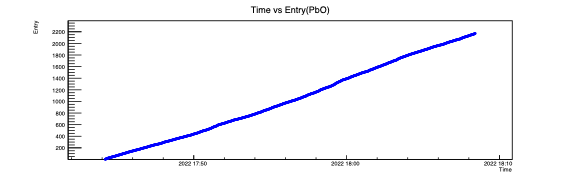
\includegraphics[width=200pt]{./Figure/EBES/Time_PbO.png}%.5\linewidth]{./Figure/DLAnalysis/Input2.png}
  			\caption{}
  			\label{fig:sfig1}
 		\end{center}
	\end{subfigure}
	\begin{subfigure}{.5\textwidth}
		\begin{center}
			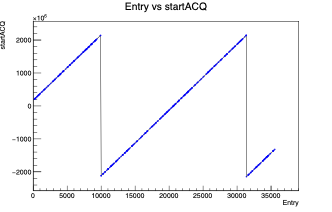
\includegraphics[width=250pt]{./Figure/EBES/Time_SiW.png}%.5\linewidth]{./Figure/DLAnalysis/Input2.png}
			\caption{}
			\label{fig:sfig2}
		\end{center}
	\end{subfigure}
	\caption[鉛ガラス検出器およびSiW ECALの計測時間]{鉛ガラス検出器およびSiW ECALの計測時間。(a)は鉛ガラス検出器、(b)はSiW ECALのものである。SiW ECALは$\SI{32}{bit}$ごとにループしている。}
	\label{time}
\end{figure}

SiW ECALで測定された時間を変換し、UNIX TIMEに修正した。修正後の時間測定を図\ref{time_correction}に示す。

\begin{figure}[H]
	\begin{center}
		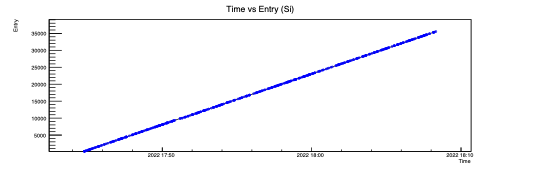
\includegraphics[width=330pt]{./Figure/EBES/SiW_time_correction.png}
		\caption[SiW ECALの変換後の計測時間]{SiW ECALの変換後の計測時間。}
		\label{time_correction}
	\end{center}
\end{figure}

鉛ガラス検出器で計測された時間と比較してもほとんど同じプロットになっている。
\end{comment}


%続いて、ビームの影響で生じるバックグラウンドについて調べるために、ビーム
%%%%%%%%%%%%%%%%%%%%%%%%%%%%%%%%%%%%%%%%%%%%%%%%%%%%%%%%%%%%%%%%%%%%%%%%%%%%%%%%%%%%%%%%%%%%%%%
%%%%%%%%%%%%%%%%
\begin{comment}
SiW ECALで測定された時間を以下の式で補正し、UNIX TIMEへと変換した。ただし、$t_bit$は
\begin{equation}

\end{equation}
\end{comment}
%%%%%%%%%%%%%%%%%


%2日間実験を行ったうち、急激に鉛検出器のADCが上昇するタイミングが何回か確認された。%ビームの偏極の様子を確認すると、



